\subsection{Case 0, $M=N$}
The results are plotted for data set S1\_Cclean. The test is performance on 144 time segment with $L_s = 516$ and $M = 27$ sensors. 

Figure \ref{fig:M=N_1} show $MSE\left(\hat{\mathbf{X}}_{\text{main}},\hat{\mathbf{X}}_{\text{ICA}}\right)$ for all segments $s$. ICA is applied on $\textbf{Y}_s$ specified by $M_= 27$ and $L_s = 516$.  Main algorithm is applied on $\textbf{Y}_s$ specified by $M=27$ and $L_s=5156$, given $\textbf{A}_{fix}$ and $N = k$ given by from ICA.
\begin{figure}[H]
    \begin{minipage}[t]{.45\textwidth}
		\centering
		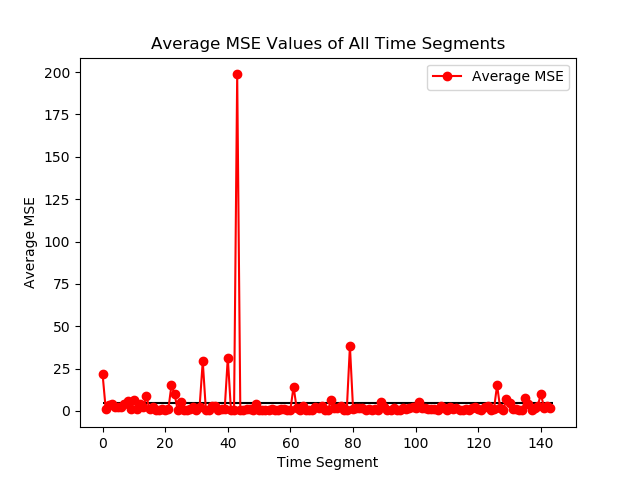
\includegraphics[scale=0.5]{figures/ch_7/average_mse_non_removed_ica}
	\caption{$MSE\left(\hat{\mathbf{X}}_{\text{main}},\hat{\mathbf{X}}_{\text{ICA}}\right)$ for all 144 segments}
	\label{fig:M=N_1}
    \end{minipage} 
    \hfill
    \begin{minipage}[t]{.45\textwidth}
        \centering
		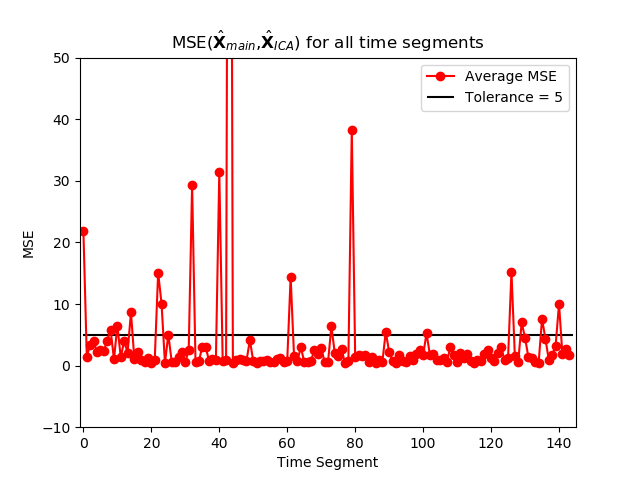
\includegraphics[scale=0.5]{figures/ch_7/average_mse_non_removed_ica_zoom.png}
	\caption{$MSE\left(\hat{\mathbf{X}}_{\text{main}},\hat{\mathbf{X}}_{\text{ICA}}\right)$ for all 144 segments. Plotted only for the y-axis interval [-10, 50] for better visualisation.}
	\label{fig:M=N_1_2}
    \end{minipage}
\end{figure}
\noindent 
 
\begin{figure}[H]
\centering
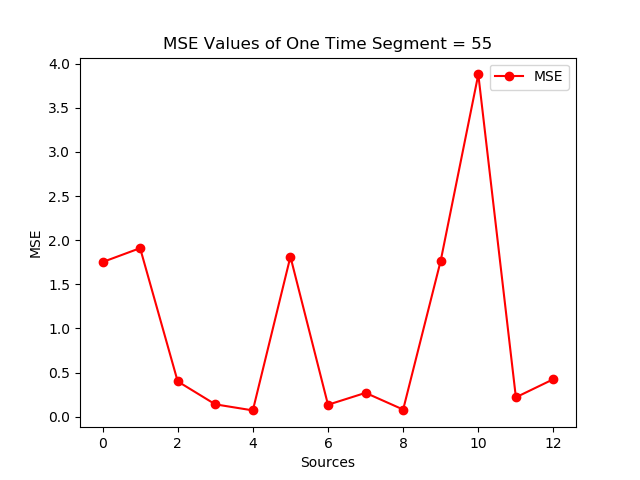
\includegraphics[scale=0.5]{figures/ch_7/mse_non_removed_ica_timeseg54.png}
\caption{$MSE\left(\hat{\mathbf{X}}_{\text{main}_{i}},\hat{\mathbf{X}}_{\text{ICA}_{i}}\right)$ for every row $i = 1, \hdots, k$ in time segment $s=56$.}
\label{fig:M=N_2}
\end{figure}
\noindent
From figure \ref{fig:M=N_1_2} it is seen that the average MSE of $\hat{\mathbf{X}}_{\text{main}}$ compared to $\hat{\mathbf{X}}_{\text{ICA}}$ mostly laid between 0 and 10. 

In figure \ref{fig:M=N_2} the MSE values of one time segment is plotted to visualize how the sources performs compared to the ICA. The time segment in interest is $s = 45$ so the segment of the 45 second in S1\_Cclean. 

From figure \ref{fig:M=N_2} it seen that the estimation of the sources in this time segment have a low MSE value. Furthermore, it is seen that for source 12-14 a high MSE value occur. This is because of how the sources are replaced to match the index of $\hat{\mathbf{X}}_{\text{ICA}}$.

The last figure illustrate the $k = 13$ sources from $\hat{\mathbf{X}}_{\text{main}}$ and $\hat{\mathbf{X}}_{\text{ICA}}$ plot on each other.
\begin{figure}[H]
    \centering
	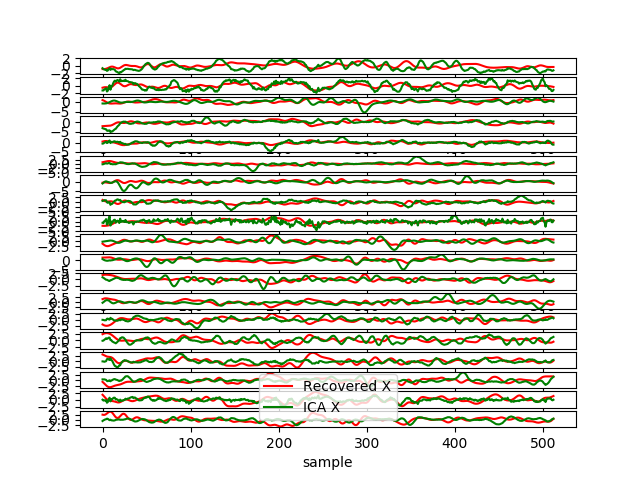
\includegraphics[scale=0.5]{figures/ch_7/Sources_M=N.png}
	\caption{Plot of the $k = 13$ sources from $\hat{\mathbf{X}}_{\text{main}}$ and $\hat{\mathbf{X}}_{\text{ICA}}$ from time segment $s = 45$ with $M=N$}
	\label{fig:M=N_3}
\end{figure} 
\noindent


%The main algorithm manage to make almost an exact recovering when looking at simpler data set for $M=N$. Figure \ref{fig:M=N_test} illustrate such recovering.
%\begin{figure}[H]
%    \centering
%	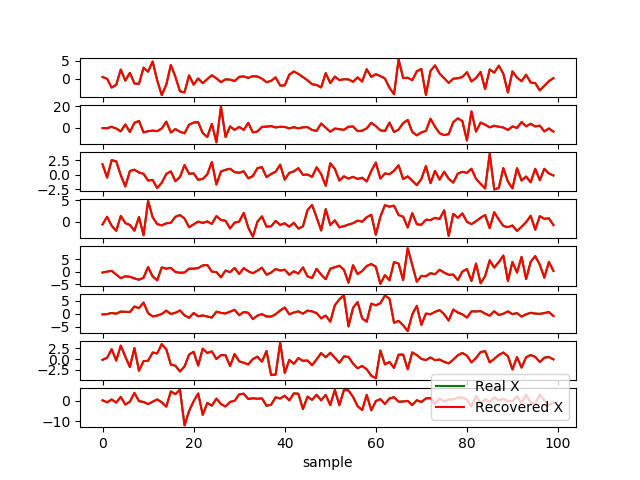
\includegraphics[scale=0.5]{figures/ch_7/M=N_test.png}
%	\caption{This is an example from the autoregressive data set where the system specification are $M=N$. Exact recovering when $M=N$ with only a MSE of 3.78e-28.}
%	\label{fig:M=N_test}
%\end{figure}



\subsection{Test on EEG Data Set with $\frac{1}{3} M<N$}
For this test the S1\_Cclean EEG data set will be used and case of interest is when $\frac{1}{3} M < N$, every third sensors is removed from S1\_Cclean EEG data set. The test is performance on 144 time segment with $L_s = 516$ and $M = 18$ sensors. From ICA 144 different $k$ values will represent the activation of sources. The obtain source matrices will only consists of the active sources.
The aim of this test is to see if one still can recover the same sources as the in the case of $M=N$. It is expected that a higher MSE will be seen.

Figure \ref{fig:M<N_1} visualize the average MSE values obtain from $\hat{\mathbf{X}}_{\text{main}}$ and $\hat{\mathbf{X}}_{\text{ICA}}$, one MSE value per time segment.
\begin{figure}[H]
    \begin{minipage}[t]{.45\textwidth}
		\centering
		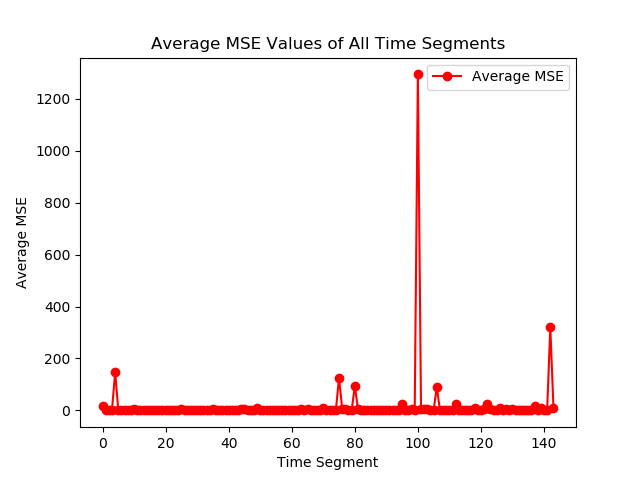
\includegraphics[scale=0.5]{figures/ch_7/AveMSE_3M_N.png}
	\caption{Average MSE of the main algorithm with $M=18$, $L = 516$ and a different $k$ for each time segment. The main algorithm and ICA is used on the S1\_Cclean EEG data set.}
	\label{fig:M<N_1}
    \end{minipage} 
    \hfill
    \begin{minipage}[t]{.45\textwidth}
        \centering
		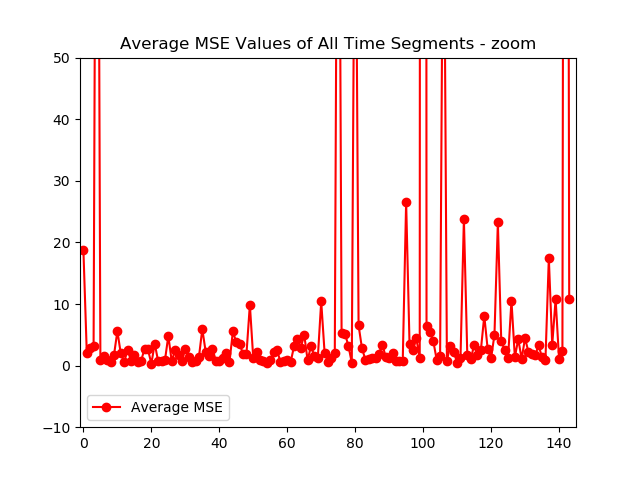
\includegraphics[scale=0.5]{figures/ch_7/AveMSE_3M_N_zoom.png}
	\caption{Average MSE of the main algorithm with $M=18$, $L = 516$ and a different $k$ for each time segment. The main algorithm and ICA is used on the S1\_Cclean EEG data set -- zoom version.}
	\label{fig:M<N_1_2}
    \end{minipage}
\end{figure}
\noindent 
 
\begin{figure}[H]
\centering
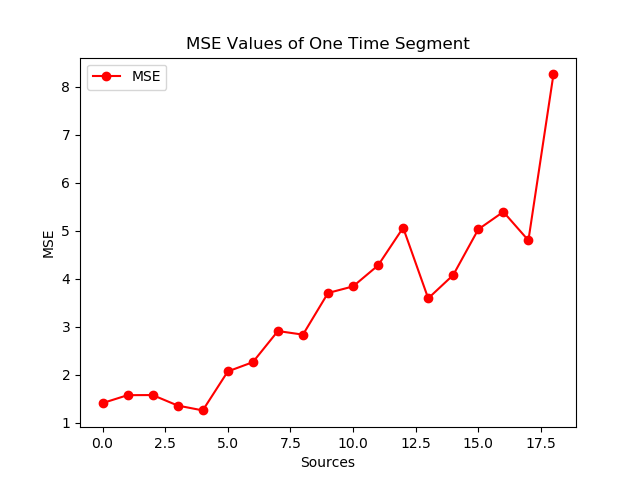
\includegraphics[scale=0.5]{figures/ch_7/MSE_3M_N.png}
	\caption{MSE of the main algorithm with $M=18$, $L = 516$ and $k=13$ for time segment $s=45$. The main algorithm and ICA is used on the S1\_Cclean EEG data set.}
\label{fig:M<N_2}
\end{figure}
\noindent
From figure \ref{fig:M<N_1_2} it is seen that the average MSE of $\hat{\mathbf{X}}_{\text{main}}$ compared to $\hat{\mathbf{X}}_{\text{ICA}}$ mostly laid between 0 and 10 but a mosre higher MSE tendency can be seen compared to the MSE from $M=N$. 

In figure \ref{fig:M<N_2} the MSE values of one time segment is plotted to visualize how the sources performs compared to the ICA. The time segment in interest is $s = 45$ so the segment of the 45 second in S1\_Cclean. 
From figure \ref{fig:M<N_2} it seen that the estimation of the sources in this time segment have a higher MSE value compared to \ref{fig:M=N_2}. This verifies the expectation that the less sensors a higher MSE values will occur.

The last figure illustrate the $k = 13$ sources from $\hat{\mathbf{X}}_{\text{main}}$ and $\hat{\mathbf{X}}_{\text{ICA}}$ plot on each other.
\begin{figure}[H]
    \centering
	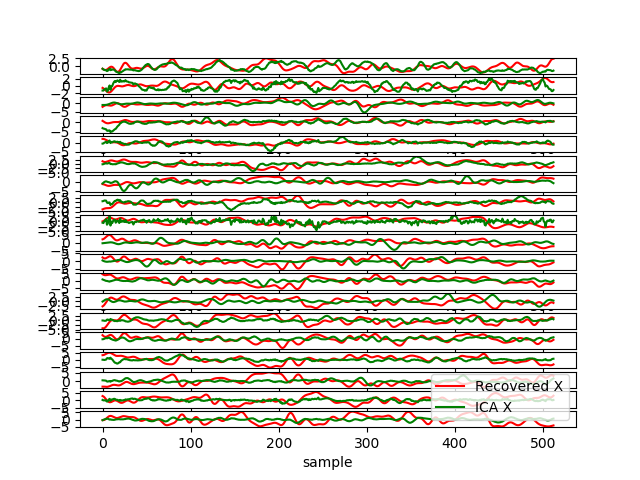
\includegraphics[scale=0.5]{figures/ch_7/Sources_3M_N.png}
	\caption{Plot of the $k = 13$ sources from $\hat{\mathbf{X}}_{\text{main}}$ and $\hat{\mathbf{X}}_{\text{ICA}}$ from time segment $s = 45$ with $\frac{1}{3} M<N$}
	\label{fig:M<N_3}
\end{figure} 
\noindent

\subsection{Test on EEG Data Set with $\frac{1}{2} M<N$}
For this test the S1\_Cclean EEG data set will be used and case of interest is when $\frac{1}{2} M < N$, every second sensors is removed from S1\_Cclean EEG data set. The test is performance on 144 time segment with $L_s = 516$ and $M = 13$ sensors. From ICA 144 different $k$ values will represent the activation of sources. The obtain source matrices will only consists of the active sources.
The aim of this test is the same as the previous, to see if one still can recover the same sources as the in the case of $M=N$. It is still expected to see a higher MSE.

Figure \ref{fig:M<<N_1} visualize the average MSE values obtain from $\hat{\mathbf{X}}_{\text{main}}$ and $\hat{\mathbf{X}}_{\text{ICA}}$, one MSE value per time segment.

\begin{figure}[H]
    \begin{minipage}[t]{.45\textwidth}
		\centering
		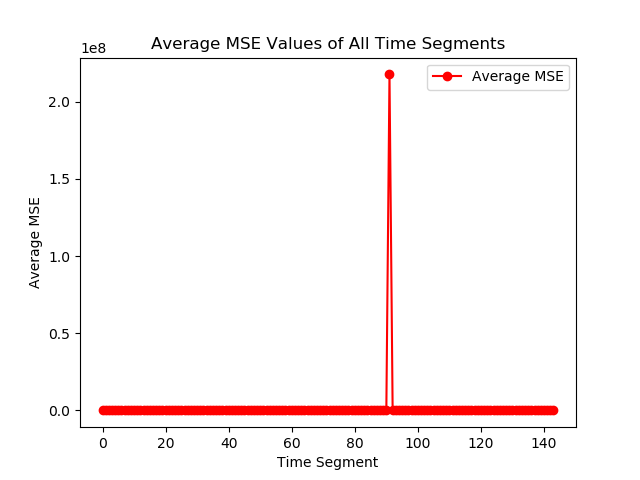
\includegraphics[scale=0.5]{figures/ch_7/AveMSE_2M_N.png}
	\caption{Average MSE of the main algorithm with $M=13$, $L = 516$ and a different $k$ for each time segment. The main algorithm and ICA is used on the S1\_Cclean EEG data set.}
	\label{fig:M<<N_1}
    \end{minipage} 
    \hfill
    \begin{minipage}[t]{.45\textwidth}
        \centering
		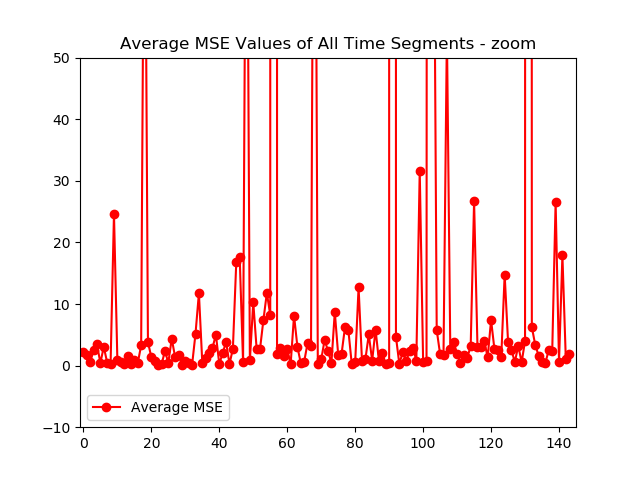
\includegraphics[scale=0.5]{figures/ch_7/AveMSE_2M_N_zoom.png}
	\caption{Average MSE of the main algorithm with $M=13$, $L = 516$ and a different $k$ for each time segment. The main algorithm and ICA is used on the S1\_Cclean EEG data set -- zoom version.}
	\label{fig:M<<N_1_2}
    \end{minipage}
\end{figure}
\noindent

\begin{figure}[H]
\centering
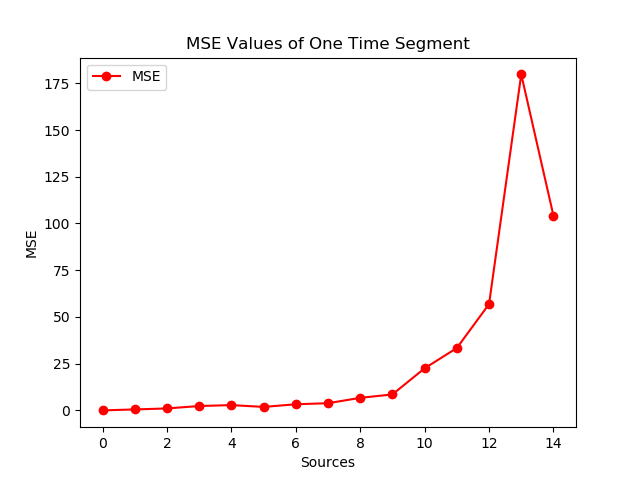
\includegraphics[scale=0.5]{figures/ch_7/MSE_2M_N.png}
\caption{MSE of the main algorithm with $M=13$, $L = 516$ and $k=13$ for time segment $s=45$. The main algorithm and ICA is used on the S1\_Cclean EEG data set.}
	\label{fig:M<<N_2}
\label{fig:M<N_2}
\end{figure}
\noindent
From figure \ref{fig:M<<N_1_2} it is seen that the average MSE of $\hat{\mathbf{X}}_{\text{main}}$ compared to $\hat{\mathbf{X}}_{\text{ICA}}$ mostly laid between 0 and 10. 

In figure \ref{fig:M<<N_2} the MSE values of one time segment is plotted to visualize how the sources performs compared to the ICA. The time segment in interest is $s = 45$ so the segment of the 45 second in S1\_Cclean. 
From figure \ref{fig:M<<N_2} it seen that the estimation of the sources in this time segment have a generally low MSE value and is almost the same compared to \ref{fig:M=N_2}. 

The last figure illustrate the $k = 13$ sources from $\hat{\mathbf{X}}_{\text{main}}$ and $\hat{\mathbf{X}}_{\text{ICA}}$ plot on each other.
\begin{figure}[H]
    \centering
	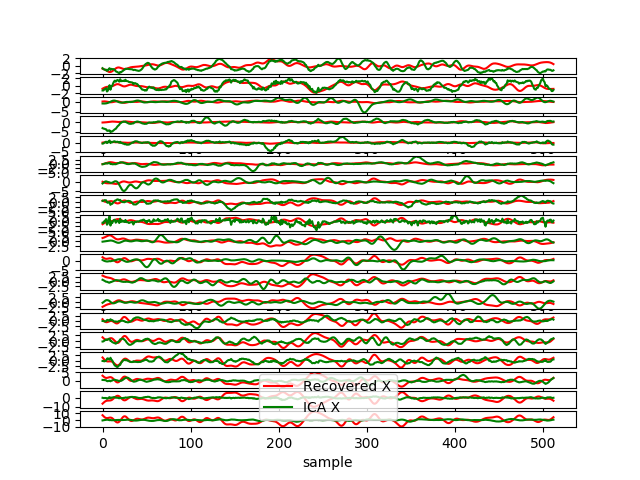
\includegraphics[scale=0.5]{figures/ch_7/Sources_2M_N.png}
	\caption{Plot of the $k = 13$ sources from $\hat{\mathbf{X}}_{\text{main}}$ and $\hat{\mathbf{X}}_{\text{ICA}}$ from time segment $s = 45$ with $\frac{1}{2} M<N$}
	\label{fig:M<<N_3}
\end{figure} 
\noindent
